\documentclass[11pt,a4paper]{article}

\def\nyear {2025}
\def\nterm {Winter}
\def\nlecturer {}
\def\ncourse {Riemann Surfaces}

\usepackage{blochsphere}
\makeatletter

% packages
\usepackage{amssymb,amsfonts,amsmath,calc,tikz,pgfplots,geometry,mathtools}
\usepackage{color}   % May be necessary if you want to color links
\usepackage[hidelinks]{hyperref}
\usepackage{forest}
\usepackage{commath} % ew
\usepackage{esdiff}
\usepackage{amsthm}
\usepackage{fancyhdr}
\usepackage{bm}
\usepackage{witharrows}
\usepackage{bookmark}
\usepackage{tikz-cd}
\usepackage{bbm}
\usepackage{textcomp}
\usepackage{gensymb}
\usepackage{cleveref}

% tikz libraries
\usetikzlibrary{positioning}
\usetikzlibrary{matrix}
\usetikzlibrary{arrows}
\usetikzlibrary{arrows.meta}
\usetikzlibrary{decorations.markings}

% Page style setup
\pagestyle{fancy}
\geometry{margin=1in}
\pgfplotsset{compat=1.18}
\setlength{\headheight}{14.6pt}
\addtolength{\topmargin}{-1.6pt}
\hypersetup{
    colorlinks=false,
    linktoc=section,
    linkcolor=black,
}

%% maketitle setup
\ifx \nauthor\undefined
  \def\nauthor{yehelip}
\else
\fi

\ifx \ncoursehead \undefined
\def\ncoursehead{\ncourse}
\fi

\lhead{\emph{\nouppercase{\leftmark}}}
\ifx \nextra \undefined
  \rhead{
    \ifnum\thepage=1
    \else
      \ncoursehead
    \fi}
\else
  \rhead{
    \ifnum\thepage=1
    \else
      \ncoursehead \ (\nextra)
    \fi}
\fi

\let\@real@maketitle\maketitle
\renewcommand{\maketitle}{\@real@maketitle\begin{center}
\begin{minipage}[c]{0.9\textwidth}\centering\footnotesize
These notes are not endorsed by the lecturers.
I have revised them outside lectures to incorporate supplementary explanations,
clarifications, and material for fun.
While I have strived for accuracy, any errors or misinterpretations 
are most likely mine.
\end{minipage}\end{center}}

% theorem environments
\theoremstyle{definition}
\newtheorem{definition}{Definition}[section]
\newtheorem{remark}{Remark}[section]
\newtheorem{example}{Example}[section]
\newtheorem{exercise}{Exercise}[section]
\newtheorem{paradox}{Paradox}[section]
\newtheorem*{solution}{Solution}
\theoremstyle{plain}
\newtheorem{theorem}{Theorem}[section]
\newtheorem{proposition}[theorem]{Proposition}
\newtheorem{lemma}[theorem]{Lemma}
\newtheorem{corollary}[theorem]{Corollary}

% tikz customization
\pgfarrowsdeclarecombine{twolatex'}{twolatex'}{latex'}{latex'}{latex'}{latex'}
\tikzset{->/.style = {decoration={markings,
                                  mark=at position 1
                                  with {\arrow[scale=2]{latex'}}},
                      postaction={decorate}}}
\tikzset{<-/.style = {decoration={markings,
                                  mark=at position 0 with {\arrowreversed[scale=2]{latex'}}},
                      postaction={decorate}}}
\tikzset{<->/.style = {decoration={markings,
                                   mark=at position 0 with {\arrowreversed[scale=2]{latex'}},
                                   mark=at position 1 with {\arrow[scale=2]{latex'}}},
                       postaction={decorate}}}
\tikzset{->-/.style = {decoration={markings,
                                   mark=at position #1 with {\arrow[scale=2]{latex'}}},
                       postaction={decorate}}}
\tikzset{-<-/.style = {decoration={markings,
                                   mark=at position #1 with {\arrowreversed[scale=2]{latex'}}},
                       postaction={decorate}}}
\tikzset{->>/.style = {decoration={markings,
                                  mark=at position 1 with {\arrow[scale=2]{latex'}}},
                      postaction={decorate}}}
\tikzset{<<-/.style = {decoration={markings,
                                  mark=at position 0 with {\arrowreversed[scale=2]{twolatex'}}},
                      postaction={decorate}}}
\tikzset{<<->>/.style = {decoration={markings,
                                   mark=at position 0 with {\arrowreversed[scale=2]{twolatex'}},
                                   mark=at position 1 with {\arrow[scale=2]{twolatex'}}},
                       postaction={decorate}}}
\tikzset{->>-/.style = {decoration={markings,
                                   mark=at position #1 with {\arrow[scale=2]{twolatex'}}},
                       postaction={decorate}}}
\tikzset{-<<-/.style = {decoration={markings,
                                   mark=at position #1 with {\arrowreversed[scale=2]{twolatex'}}},
                       postaction={decorate}}}

\pgfarrowsdeclare{biggertip}{biggertip}{%
  \setlength{\arrowsize}{1pt}
  \addtolength{\arrowsize}{.1\pgflinewidth}
  \pgfarrowsrightextend{0}
  \pgfarrowsleftextend{-5\arrowsize}
}{%
  \setlength{\arrowsize}{1pt}
  \addtolength{\arrowsize}{.1\pgflinewidth}
  \pgfpathmoveto{\pgfpoint{-5\arrowsize}{4\arrowsize}}
  \pgfpathlineto{\pgfpointorigin}
  \pgfpathlineto{\pgfpoint{-5\arrowsize}{-4\arrowsize}}
  \pgfusepathqstroke
}
\tikzset{
	EdgeStyle/.style = {>=biggertip}
}

\tikzset{circ/.style = {fill, circle, inner sep = 0, minimum size = 3}}
\tikzset{scirc/.style = {fill, circle, inner sep = 0, minimum size = 1.5}}
\tikzset{mstate/.style={circle, draw, black, text=black, minimum width=0.7cm}}

\tikzset{eqpic/.style={baseline={([yshift=-.5ex]current bounding box.center)}}}

\definecolor{mblue}{rgb}{0.2, 0.3, 0.8}
\definecolor{morange}{rgb}{1, 0.5, 0}
\definecolor{mgreen}{rgb}{0, 0.4, 0.2}
\definecolor{mred}{rgb}{0.5, 0, 0}

% topology
\newcommand{\Cells}{\text{Cells}}

% algebra
\DeclareMathOperator{\lcm}{lcm}
\DeclareMathOperator{\Out}{Out}
\DeclareMathOperator{\Aut}{Aut}
\DeclareMathOperator{\End}{End}
\DeclareMathOperator{\Inn}{Inn}
\DeclareMathOperator{\Mat}{Mat}
\DeclareMathOperator{\std}{std}
\DeclareMathOperator{\sgn}{sgn}
\DeclareMathOperator{\id}{id}
\DeclareMathOperator{\op}{op}
\DeclareMathOperator{\GL}{GL} % General linear group
\DeclareMathOperator{\SL}{SL} % Special linear group
\newcommand{\idealin}{\triangleleft}
\newcommand{\ip}[2]{\langle #1, #2 \rangle}
\newcommand{\bigslant}[2]
{{\raisebox{.2em}{$#1$}\left/\raisebox{-.2em}{$#2$}\right.}}

% analysis
\newcommand{\dx}{\dif x}
\newcommand{\dt}{\dif t}
\newcommand{\du}{\dif u}
\newcommand{\dv}{\dif v}
\newcommand{\dz}{\dif z}
\newcommand{\ds}{\dif s}
\newcommand{\dtheta}{\dif \theta}
\DeclareMathOperator{\im}{im}
\DeclareMathOperator{\cis}{cis}
\DeclareMathOperator{\Int}{Int}
\DeclareMathOperator{\diam}{diam}
\DeclareMathOperator{\supp}{supp}
\DeclareMathOperator{\Vol}{Vol} % Volume

% logic
\DeclareMathOperator{\MOD}{MOD}
\DeclareMathOperator{\Theory}{Theory}


% nice
\newcommand{\half}{\frac{1}{2}}
\newcommand{\pair}{\del}
\newcommand{\taking}[1]{\xrightarrow{#1}}
\newcommand{\inv}{^{-1}}
\newcommand{\ot}{\leftarrow}
\newcommand{\ninfty}{-\infty}
\newcommand{\floor}[1]{\left\lfloor #1 \right\rfloor}
\newcommand{\ceil}[1]{\left\lceil #1 \right\rceil}

% probability
\newcommand{\Prob}{\mathbf{P}}
\renewcommand{\vec}[1]{\boldsymbol{\mathbf{#1}}}
\DeclareMathOperator{\Bin}{Bin}
\DeclareMathOperator{\Geo}{Geo}
\DeclareMathOperator{\Poi}{Poi}
\DeclareMathOperator{\Exp}{Exp}
\DeclareMathOperator{\Var}{Var} % Variance
\DeclareMathOperator{\Cov}{Cov}

% special letters
\newcommand{\N}{\mathbb{N}}
\newcommand{\Z}{\mathbb{Z}}
\newcommand{\Q}{\mathbb{Q}}
\newcommand{\R}{\mathbb{R}}
\newcommand{\C}{\mathbb{C}}
\newcommand{\F}{\mathbb{F}}
\newcommand{\E}{\mathbb{E}}
\newcommand{\ps}{\mathcal{P}}
\newcommand{\M}{\mathcal{M}}
\renewcommand{\L}{\mathcal{L}}
\newcommand{\Omicron}{O}
\newcommand{\powerset}{\mathcal{P}}

% text
\newcommand{\st}{\text{ s.t. }}
\newcommand{\tand}{\quad \text{and} \quad}
\newcommand{\tor}{\quad \text{or} \quad}
\newcommand{\stand}{\text{ and }}
\newcommand{\stor}{\text{ or }}
\renewcommand{\tt}[1]{\textnormal{\textbf{(#1).}}} %tt=theorem title GET RID OF

% title format
\title{\textbf{\ncourse}}
\author{Based on lectures by \nlecturer \\\small Notes taken by \nauthor}
\date{\nterm\ \nyear}
\makeatother


\DeclareMathOperator{\Bih}{Bih}
\renewcommand{\H}{\mathbb H}

\begin{document}
\maketitle

% Insert cool image here

\newpage
\tableofcontents
\newpage

\section{Introduction}
\begin{definition}[Riemann surface]
    A Riemann surface is a $1$-dimensional complex manifold.
\end{definition}

\begin{definition}[Riemann surface]
    A Riemann surface is a topological space $X$ together with
    open subsets $\set{U_k}_{k \in I}$ of $X$ with
    $\cup_{k \in I} U_k = X$ together with maps $f_i \colon U_i \to \C$
    such that
    \begin{enumerate}
        \item[(1)] Each $f_i$ is a homeomorphism onto its image.
        \item[(2)] If $U_i \cap U_j \neq \emptyset$ then 
            $f_i \circ f_j^{-1} \colon 
            f_j(U_i \cap U_j) \to f_i(U_i \cap U_j)$ are \emph{biholomorphic}.
    \end{enumerate}
\end{definition}

\begin{remark}
    A function $f \colon \C \to \C$ is holomorphic at $p$ if 
    $f'(p) = \lim_{z \to p} \frac{f(z) - f(p)}{z - p}$ exists.
\end{remark}

\begin{definition}[Biholomorphism]
    A function $f \colon \C \to \C$ is called biholomorphic if it has an inverse
    and both $f$ and $f'$ are holomorphic.
\end{definition}

\begin{definition}[Atlas]
    The $\set{(U_i, f_i)}_{i \in I}$ are called an atlas of the Riemann surface.
\end{definition}

\begin{definition}[Chart]
    Each individual $(U_i, f_i)$ is called a chart of the Riemann surface.
\end{definition}

\begin{example}
    Let $U \subset \C$.
    Then $U$ can take an atlas with one chart which is the identity map.
\end{example}

\begin{example}[Riemann sphere]
    Let $X = \set{(z,t) \in \C \times \R \colon |z|^2 + t^2 = \R}$.
    We identify $\C$ with the $xy$ plane.
    Denote $N$ and $S$ the north and south poles of the sphere accordingly.
    We define $\pi_N \colon \C \to S$ such that $\pi_N$ sends each point
    $(z,t)$ on the sphere to its stereographic projection 
    from $N$ onto the plane (point $\xi$) as can be seen in the figure
    below:
    \begin{center}
      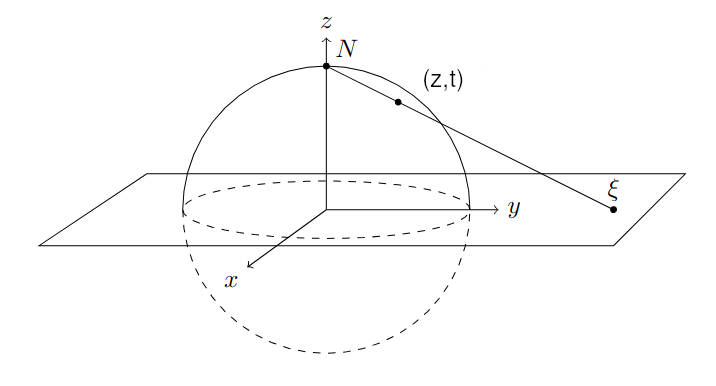
\includegraphics[scale=0.5]{RiemannSphere.png}
    \end{center}
    We can similarly define $\pi_S$ and verify that the images of the
    projections are $X \setminus \set{N}$ and $X \setminus \set{S}$
    accordingly.
    
    Now $X$ is a Riemann surface with an atlas consisting of 
    $\pi_S \colon X \setminus \set{S} \to \C$ and
    $\pi_N \colon X \setminus \set{N} \to \C$.
    We denote the Riemann sphere as $\hat{\C}$.
\end{example}

\begin{definition}[Biholomorphism of Riemann surfaces]
    Let $(X, (U_i, f_i))$, $(Y, (W_i,g_i))$ be two Riemann surfaces.
    A biholomorphism between them is a homeomorphism
    $X \xrightarrow{\phi} Y$ such that $g_i \circ \phi \circ f_i^{-1}$ 
    are biholomorphisms on their domains of definition.
\end{definition}

A main problem in Riemann surfaces was classifying certain types of 
Riemann surfaces up to biholomorphisms.

\begin{theorem}\tt{Riemann mapping theorem}
    Any two proper open simply connected subsets of $\C$ are biholomorphic.
\end{theorem}

A generalization of the Riemann mapping theorem is the uniformization theorem
proved by Kobe in 1907.

\begin{theorem}\tt{Uniformization theorem}
    Any simply connected Riemann surface is biholomorphic to one of the
    following:
    \begin{enumerate}
        \item[(1)] $\C$
        \item[(2)] $\hat{\C}$
        \item[(3)] $\H = \set{z \in \C \colon \mathrm{Im}(z) > 0}$
    \end{enumerate}
\end{theorem}

We will give a proof for this theorem in the end of the class.

A natural question that arises is what about non simply connected Riemann
surfaces?

\begin{theorem}\tt{Uniformization theorem, part II}
    Any connected Riemann surface is biholomorphic either to $\hat{\C}$
    or to a quotient of $\C$ or $\H$ by a properly discontinuous
    torsion-free subgroup of biholomorphisms.
\end{theorem}

\begin{remark}
    Biholomorphisms of $U = \C$ or $\H$ (or any subset of $\C$)
    forms a group under composition.
    We denote that group by $\Bih(U)$.
\end{remark}

\begin{definition}[Properly discontinuous group]
    A countable subgroup of $\Bih(U)$ is said to be properly discontinuous
    if for all compact $K \subseteq U$, the set 
    $\set{g \in G \colon gK \cap K \neq \emptyset}$ is finite.
\end{definition}

\begin{definition}[Torsion-free group]
    $G \subseteq \Bih(U)$ is torsion-free if $gp = p$ for some $p \in U$
    implies $g$ is the identity.
\end{definition}

\begin{remark}
  Notice that multiplication in $gp$ is the group action of $g$ on the 
  set $U$. That us $gp = g(p)$.
\end{remark}

We can know define the quotient space $\bigslant{U}{G}$ where
$p \sim q$ if there exists $g \in G$ such that $gp = q$.

Introduce a topology on $\bigslant{U}{G}$ which is the coarsest topology
such that the canonical projections $U \to \bigslant{U}{G}$ are continuous.

Under the assumptions that $G$ is properly discontinuous and torsion-free,
$\bigslant{U}{G}$ is a Riemann surface with the following charts.
By assumptions on $G$, we can find for any $p \in U$ a neighbourhood $W$ of
$p \in U$ such that $\pi \colon U \to \bigslant{U}{G}$ is a homeomorphism
onto its image when restricted to $W$.

So, restrictions of $\pi$ to these neighbourhoods $W$ give an atlas.





\end{document}
